\subsubsection{Procedure}
Per il coordinamento e le comunicazioni durante la realizzazione del progetto, il gruppo adotterà le seguenti procedure: 
\begin{itemize}
\item\textbf{comunicazione interna}: coinvolge tutti i membri del team;
\item\textbf{comunicazione esterna}: con \glo{proponente} e committente.
\end{itemize}

\paragraph{Gestione delle comunicazioni}

\subparagraph{Comunicazioni interne} \mbox{} \\
Le comunicazioni interne avvengono attraverso il canale \glo{Discord}. Quest'applicazione favorisce la collaborazione a distanza e viene utilizzata anche in ambienti aziendali. Tale software permette al team di creare uno spazio di lavoro condiviso.
\subparagraph{Comunicazioni esterne} \mbox{} \\
Le comunicazioni con utenti esterni al gruppo sono gestite dal responsabile del progetto. Le modalità utilizzate sono le seguenti: 
\begin{itemize}
\item Tramite posta elettronica (all'indirizzo \textcolor{blue}{\textbf{codebusterswe@gmail.com}}); 
\item Attraverso \glo{Skype} per i colloqui con l'azienda Zucchetti.
\end{itemize} 
\paragraph{Gestione degli incontri}
\subparagraph{Incontri interni} \mbox{} \\
Il responsabile del progetto concorda con il team gli incontri interni. Egli ha il compito di specificare le date delle riunioni nel calendario e approvare i verbali redatti. I membri del gruppo sono tenuti a partecipare alle riunioni, interagendo nei dibattiti. Affinché una riunione sia ritenuta valida, devono essere presenti almeno cinque membri del gruppo.
\subparagraph{Verbali di riunioni interne} \mbox{} \\
In occasione di ogni incontro interno viene redatto un verbale dal segretario scelto dal responsabile. Il contenuto della riunione deve essere riportato nel verbale corrispondente e approvato dal responsabile.
\subparagraph{Incontri esterni} \mbox{} \\
Il responsabile del progetto organizza gli incontri esterni con il \glo{proponente} o committente. Questi potrebbero richiedere incontri con il team; il responsabile è tenuto a proporre una data in accordo con le parti e la comunica attraverso i canali sopra citati.
\subparagraph{Verbali di riunioni esterne} \mbox{} \\
In occasione di ogni incontro esterno viene redatto un verbale da un redattore scelto dal responsabile. Il contenuto della riunione deve essere riportato nel verbale esterno corrispondente e approvato dal responsabile.
\paragraph{Gestione degli strumenti e di coordinamento}
\subparagraph{Ticketing} \mbox{} \\
Il ticketing permette ai membri del gruppo di rimanere aggiornati sullo stato delle attività in corso. Il responsabile assegna compiti ai membri del gruppo e controlla l'andamento delle \glo{tasks} assegnate. Lo strumento di ticketing scelto è \glo{Planner}: si tratta di un'applicazione \glo{multi-piattaforma}, in cui è visibile a tutti i membri del team lo stato di avanzamento dei compiti assegnati, con la possibilità di aggiungerne di nuovi. 

\paragraph{Gestione dei rischi}
Il responsabile è tenuto a individuare i rischi e renderli noti; tale attività verrà documentata nel \PdP{}. La procedura per la gestione dei rischi è: 
\begin{figure}[!htb]
   %\begin{minipage}{0.6\textwidth}
     \centering
     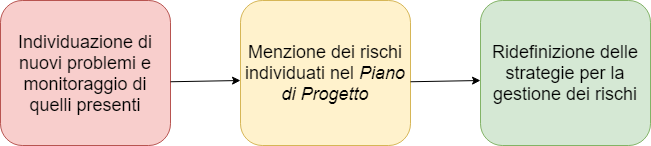
\includegraphics[scale=0.6]{Images/GestioneRischi.png}
     \caption{Procedura per la gestione dei rischi}
   %\end{minipage}
\end{figure}

\subparagraph{Codifica dei rischi} \mbox{} \\
I rischi sono codificati nel modo seguente: 
\begin{center}
\textbf{R[Categoria][Numero]}
\end{center}
Dove:
\begin{itemize}
	\item \textbf{[Categoria]}: indica la classificazione del rischio e può assumere tre valori:
	\begin{itemize}
		\item  \textbf{T}: rischi tecnologici; 
		\item \textbf{O}: rischi organizzativi;
		\item   \textbf{I}: rischi interpersonali.
	\end{itemize}
	\item \textbf{[Numero]}: è un numero progressivo che identifica univocamente il rischio all'interno di una categoria
\end{itemize}

\subsubsection{Metriche}
Il processo di gestione organizzativa non fa uso di metriche qualitative particolari.

\subsubsection{Strumenti}
Gli strumenti utilizzati in questo processo comprendono:
\begin{itemize}
	\item \textbf{Github}: piattaforma che permette la condivisione in remoto di tutti i file prodotti e la creazione di una storia per ciascuno di questi file;
	\begin{center}
		\textcolor{blue}{\url{https://github.com/}}
	\end{center}
	\item \textbf{Git}: sistema di controllo delle versioni;
	\begin{center}
		\textcolor{blue}{\url{https://git-scm.com/}}
	\end{center}
	\item \textbf{Telegram}: applicazione di messaggistica per la comunicazione rapida e la gestione del gruppo;
	\begin{center}
		\textcolor{blue}{\url{https://telegram.org/}}
	\end{center}
	\item \textbf{Discord}: applicazione \glo{multipiattaforma} utilizzata per le riunioni interne;
	\begin{center}
		\textcolor{blue}{\url{https://discord.com/}}
	\end{center}
	\item \textbf{Skype}: applicazione che consente di effettuare delle videoconferenze, utilizzata per la comunicazione con il \glo{proponente};
	\begin{center}
		\textcolor{blue}{\url{https://www.skype.com/it/}}
	\end{center}
	\item \textbf{Google Drive}: server per la condivisione rapida di alcune documentazioni che possono essere utili riguardo l'attività in svolgimento;
	\begin{center}
		\textcolor{blue}{\url{https://www.google.com/intl/it_it/drive/}}
	\end{center}
	\item \textbf{Microsoft Planner}: piattaforma per la gestione dei compiti in svolgimento, svolti e da svolgere. Permette al gruppo di rispettare gli incrementi e le scadenze dettate dal \PdP.
	\begin{center}
		\textcolor{blue}{\url{https://www.microsoft.com/it-it/microsoft-365/business/task-management-software}}
	\end{center}
\end{itemize}